\documentclass[a4paper,11pt]{ltjsarticle}
% 数式
\usepackage{amsmath,amsfonts}
\usepackage{bm}
% 画像
\usepackage{graphicx}
\usepackage{circuitikz}
\usepackage{amsmath,amssymb}
\usepackage{siunitx}
\usepackage{float}
\usepackage{tikz}
\usepackage{askmaps}
\usepackage{multirow}
\usepackage{bigstrut}
\usepackage{slashbox}
\usepackage{rotating}
\usepackage{listings}
% 数式
\usepackage{physics}
\usepackage{mathtools}
% 画像
\usepackage{subcaption}
% 表
\usepackage{makecell}
% その他
\usepackage{url}
\usepackage{ascmac}
\usepackage{cases}
\usepackage{here}
\usepackage{upgreek}
% 日本語対応
\usepackage{luatexja}
\usepackage{luatexja-fontspec}

\AtBeginDocument{\RenewCommandCopy\qty\SI}


\definecolor{commentgreen}{RGB}{0,200,0}
\definecolor{eminence}{RGB}{120,80,250}
\definecolor{weborange}{RGB}{255,165,0}
\definecolor{frenchplum}{RGB}{10,150,200}
\definecolor{commentgreen}{RGB}{0,200,0}
\definecolor{eminence}{RGB}{120,80,250}
\definecolor{weborange}{RGB}{255,165,0}
\definecolor{frenchplum}{RGB}{10,150,200}

\lstset{
        language = {C},
        basicstyle = \ttfamily\small,
        keywordstyle=\color{eminence}\ttfamily\bfseries,
        commentstyle=\color{commentgreen}\textit,
    identifierstyle=\color{black}\ttfamily,
        xleftmargin=.35in,
        frame=lines,
    showstringspaces=false,
        numbers=left,
        stepnumber = 1,
        breaklines=true,
        numberstyle = \ttfamily\normalsize,
    tabsize=4,  
        emph={int, int8_t, int16_t, int32_t, int64_t, uint8_t, uint16_t, uint32_t, uint64_t, char, double, float, unsigned, void, bool},
        emphstyle={\color{blue}}, 
        morekeywords={>, <, ., ;, +, -, *, /, !, =, ~},
        breakindent = 10pt, 
        framexleftmargin=10mm, 
        columns=fixed,
        basewidth=0.5em,
        }

% 特定のスタイル設定
\lstdefinestyle{customtxt}{
  basicstyle=\ttfamily\footnotesize,
  backgroundcolor=\color{lightgray},
  frame=single,
  breaklines=true,
  columns=fullflexible,
  showspaces=false,
  showstringspaces=false,
  showtabs=false,
  tabsize=4,
}

\newcommand{\fig}[4]{
    \begin{figure}[htbp]
      \centering
      \includegraphics{./image/#1}
      \caption{#2}
      \label{fig:#3}
    \end{figure}
  }
\begin{document}



\section{目的}
減算回路のリバースエンジニアリングを行い、その動作原理を真理値表の作成、回路図の作成を通して理解する。
\section{原理}
今回実験で必要な知識について説明を行う。
\subsection{補数}
補数とは、ある数値とその数値を足すとちょうど繰り上がる数字のことを指す。
例えば10進数では、$69$に対する補数は$(100 - 69) = 31$である。
今回では0から7の数字を扱うため、8進数を用いて論理式の計算を行い、
回路上での論理回路では2進数を用いて計算を行う。
8進数での補数表現では、$n$に対する補数は$(8^m - n)$である。$m$は桁数である
2進数での補数表現は、$n$に対する補数は$(2^m - n)$である。$m$は桁数である。
この補数を求める操作は、ビット反転と1の加算を行うことで求めることができる。動作原理として、$n$に対する進数
から1を引いた進数では値を桁上がりをしない範囲で最大にするものであるので、$2^m$から$n$を引いた値を求めることで補数を求めることができる。
これを二進数で行うとビットの反転であり、2の補数にするためには値を1加算することで求めることができることがわかる。
例えば、$1 - 5$を行う場合には、5の補数 + 1を行うことで求めることができる。5の補数は$(2^3 - 5)_{10}= (3)_{10}$または、$(101)$を反転して$(010)$となる。これに$(001)_2$を足すと$(011)_2 = (3)_{10}$であるため、$(3 + 1)_{10} = (4)_{10}$となる。
\subsection{減算}
減算を行うときには補数を使用する。例えば$1 - 5$を行う場合には、$1 + (2^3 - 5) = 1 + 3$となる。補数を使った計算の場合符号が$m$の次のビットに現れて、$1$の場合は
正の数であることを示し、$0$の場合は負の数であることを示す。例として$5 - 1$を行うと$(1)_2$を補数にして$ (101)_2 + (111)_2 = (1100)_2$となり、4bit目に符号が現れる。
原理として、$a - b \geq 0$の場合$ a + (8 - b) \geq 8$となる。そのため、4bit目が1になる。逆に$a - b < 0$の場合、$a + (8 - b) < 8$となる。そのため、4bit目が0になる。
\subsection{計算結果が補数になる原理}
減算の原理を示したが、$(1-6)_{10}$の計算を行うとき、補数と加算を使った計算をすると計算結果が補数となる。
このようになる条件としては、減算の結果が負の数になるときである。$(1 - 6)_{10}$の例で示すと、$(001)_2 + (010)_2 = (011)_2$となる。この結果は$(3)_{10}$であるが、これは$-5$の補数である。
これを二進数の絶対値に戻すには$(0)_{10} -(- 5)_{10}$を行うとできる。$(011)_2$の補数は$(101)_2 = (5)_{10}$となるので、$(0)_{10} + (5)_{10} = (5)_{10} $となり、絶対値に直すことが出来る。
\subsection{加算器}
二進数の加算を行う方法について説明をする。各桁の足し算だけを考えたときの真理値表を表\ref{tab:halfadd}に示す。
Cは繰り上がりの出力を示し、Sは各桁の和を示す。この真理値表から論理式を求めると、$C = A \cdot B$、$S = A \oplus B$となる。これを半加算器と呼ぶ。
これをすべての桁を包括した演算に拡張して考えると、繰り上がりの計算を行う必要がある。
$A+B$を行った後に、前の桁の繰り上がりを足すことにより、全体の和を求めることができる。
そのために、半加算器を二つ用いる。1個目の半加算器の$S$の出力を2個目の半加算器の$A$に入力し、前の繰り上がりの$C$を2個目の半加算器の$B$に入力することで、$A + B + C$を行うことが出来る。
そして、二つの半加算器の$C$を$OR$演算したものを全加算器と呼ぶ。
$OR$演算をする理由としては$A B C$のどれか二つ以上が1のときに繰り上がりが発生するため、
繰り上がりの出力二つを$OR$演算することで、繰り上がりの出力を行うことが出来る。
\begin{table}[htbp]
    \centering
    \caption{半加算器の真理値表}
    \begin{tabular}{|c|c|c|c|}
        \hline
        $A$ & $B$ & $C$ & $S$ \\
        \hline
        0 & 0 & 0 & 0 \\
        0 & 1 & 0 & 1 \\
        1 & 0 & 0 & 1 \\
        1 & 1 & 1 & 0 \\
        \hline
    \end{tabular}
    \label{tab:halfadd}
\end{table}
\section{実験方法}
リバースエンジニアリングを行う手順を説明する。
\subsection{真理値表の作成}
減算回路の真理値表を作成するために、減算基板確認用基板を用いて入力を行い、セレクター基盤を経由してデコード回路に信号を入力させて、真理値表を作成する。
また、減算回路の基板にはICがついてないため、ICの配置を確認し、基板にICを取り付ける。
ICの場所を画像\ref{fig:ic}に示す。また、ICの取り付ける場所を表\ref{tab:ic}に示す。
\begin{figure}[htbp]
    \centering
    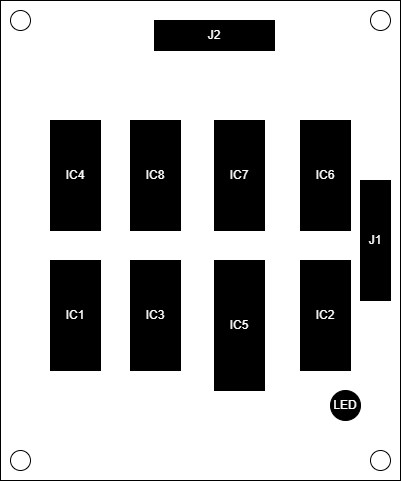
\includegraphics[width=0.5\columnwidth]{./image/ic.drawio.png}
    \caption{ICの配置}
    \label{fig:ic}
\end{figure}
\begin{table}[htbp]
    \centering
    \caption{ICの配置}
    \begin{tabular}{|c|c|}
        \hline
        IC番号 & IC名 \\
        \hline
        IC1 & 74LS04 \\
        IC2 & 74LS08 \\
        IC3 & 74LS08 \\
        IC4 & 74LS32 \\
        IC5 & 74LS83 \\
        IC6 & 74LS86 \\
        IC7 & 74LS86 \\
        IC8 & 74LS86 \\
        \hline
    \end{tabular}
    \label{tab:ic}
\end{table}
\subsection{テスターを用いて回路図を作成する}
テスターから電圧を印加させて回路の導通を確認し、導通しているピンを基に回路図の作成を行う。
\section{結果}
実験方法で示した通りに行った実験の結果を示す。
\subsection{真理値表}
真理値表を表\ref{tab:truth}に示す。
\begin{table}[htbp]
    \centering
    \caption{真理値表}
    \begin{tabular}{c|c|c}
        \hline
        $A < B$ & $C$ & $LED$ \\
        \hline
        0 & A - B & 1 \\
        1 & B - A & 0 \\
        \hline
        \hline
        $A = B$ & $C$ & $LED$ \\
        \hline
        0 & $|A - B|$ & * \\
        1 & 0 & 1 \\
        \hline
    \end{tabular}
    \label{tab:truth}
\end{table}
\subsection{回路図}
回路図を図\ref{fig:circ}に示す。
\begin{figure}[htbp]
    \centering
    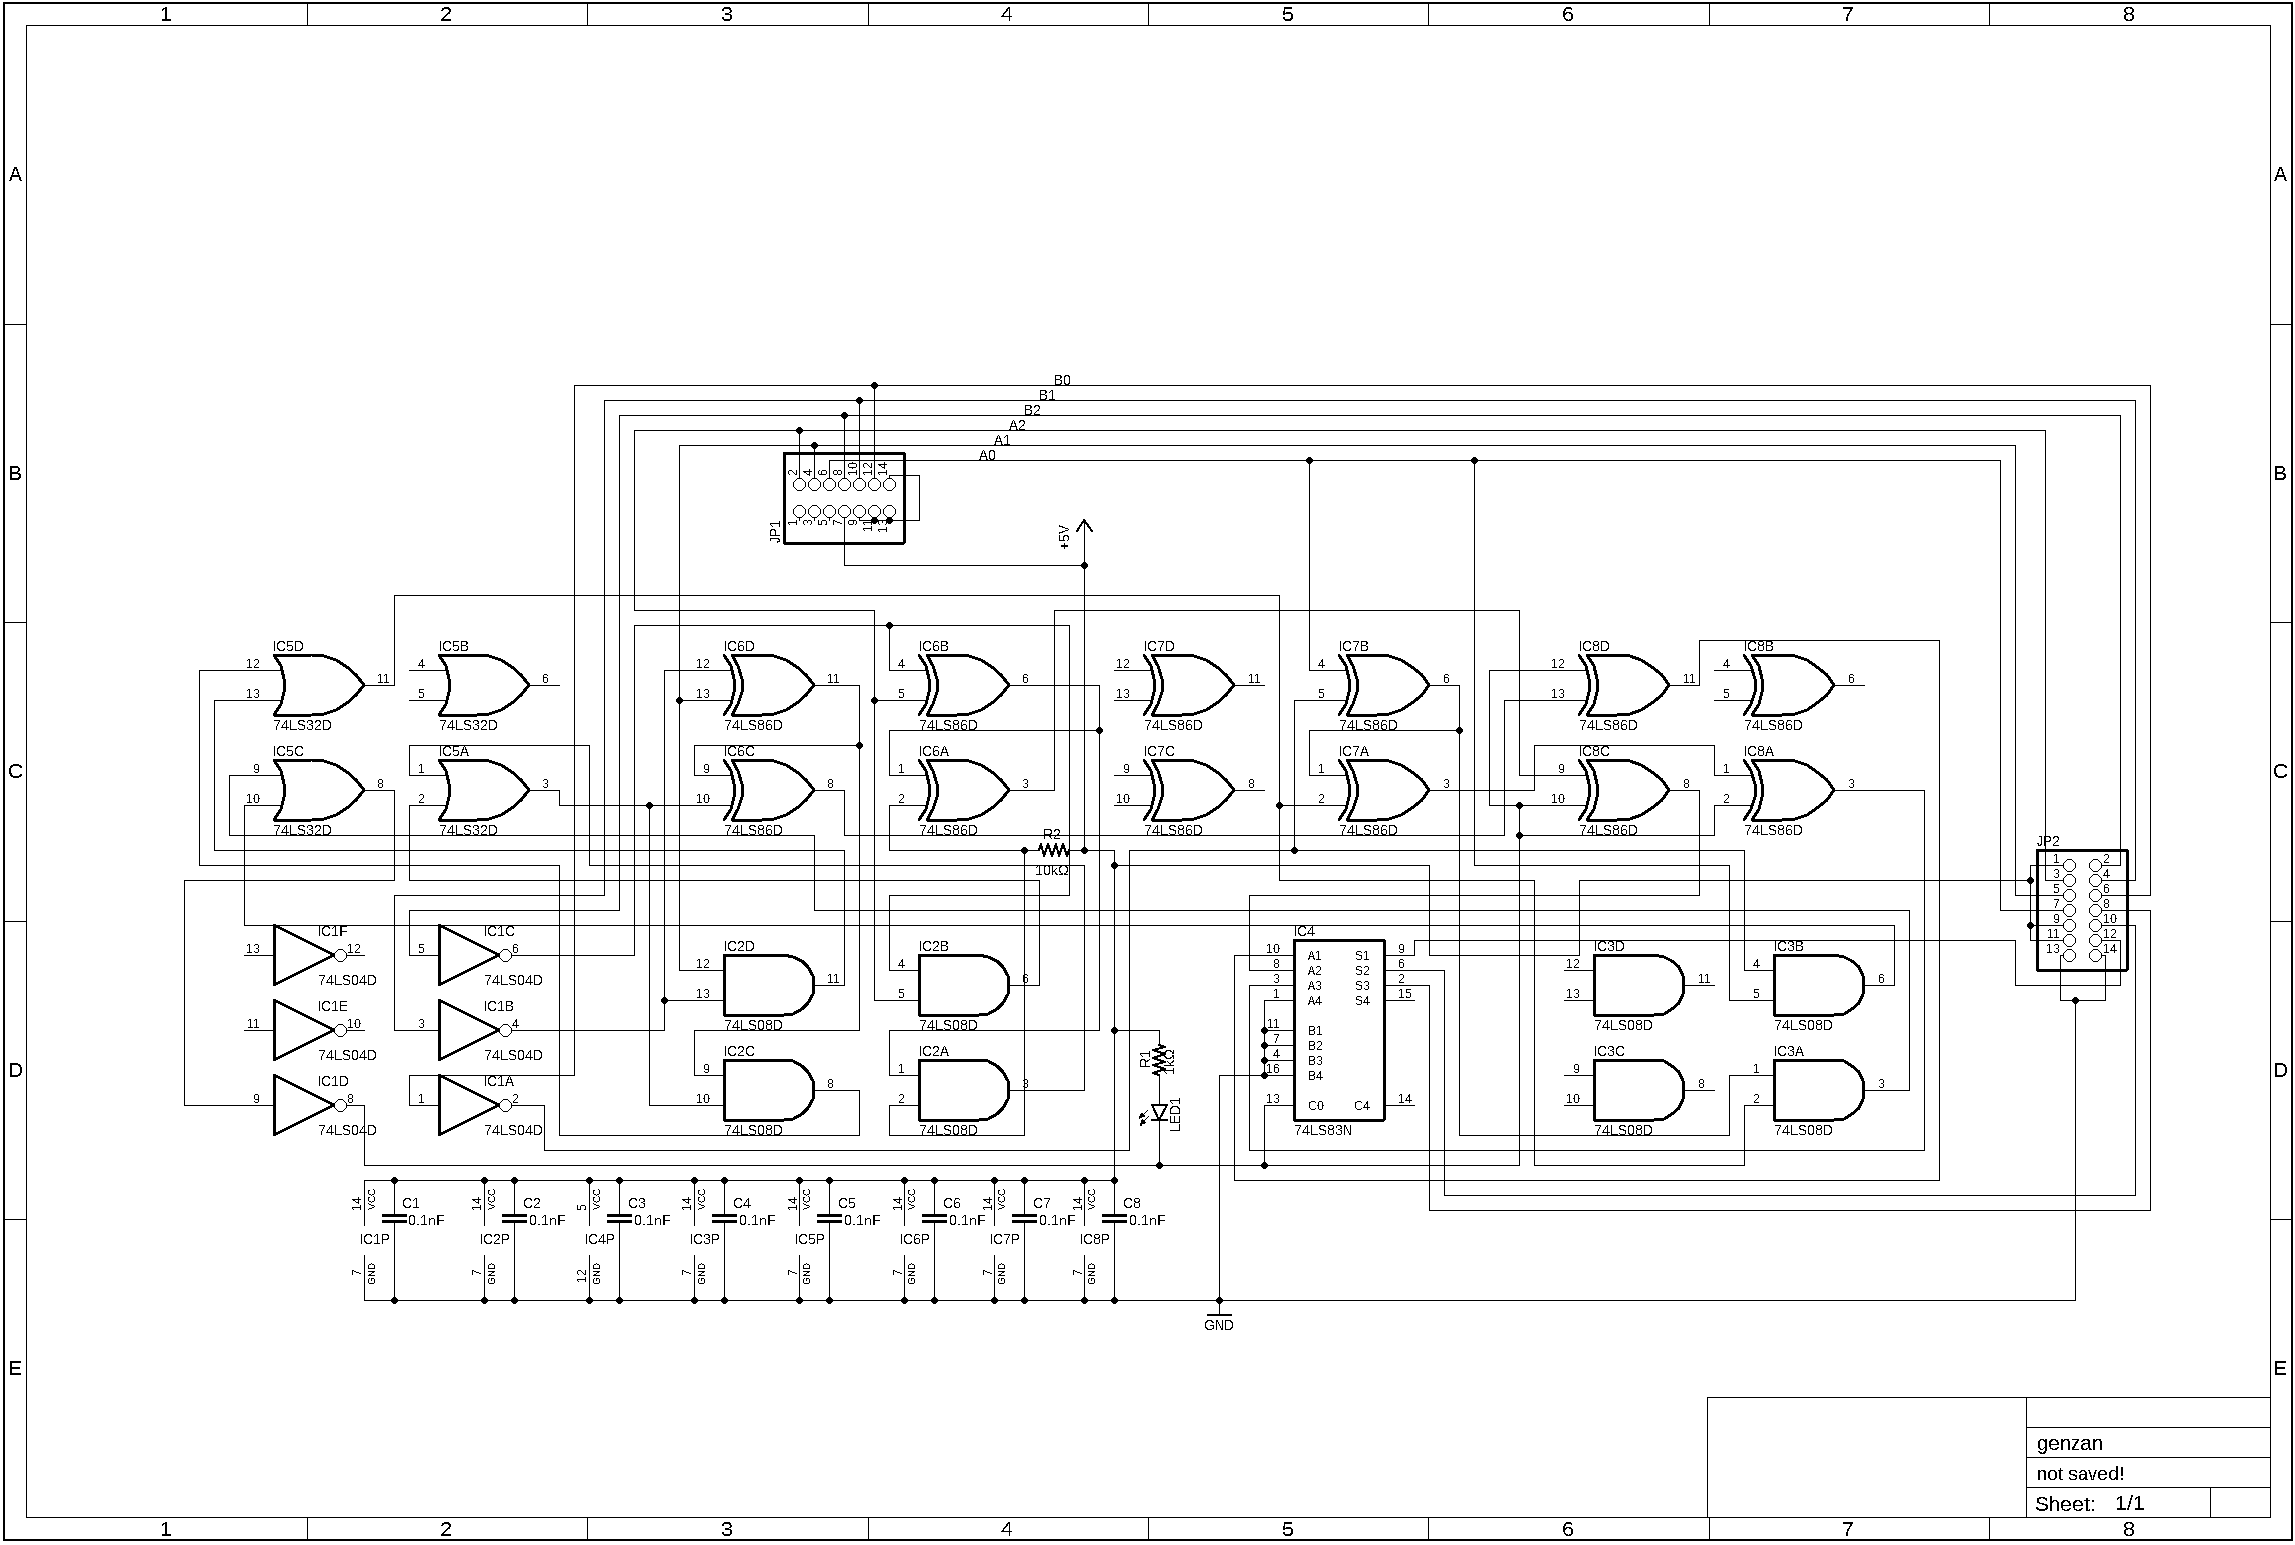
\includegraphics[angle=90,width=\columnwidth]{./image/genzan.png}
    \caption{回路図}
    \label{fig:circ}
\end{figure}
\newpage
\section{考察}
減算回路のリバースエンジニアリングを行った結果御もとに考察を書いていく。
\subsection{真理値表}
LEDの出力結果が演算結果が正の値のときに点灯になった理由として、原理で説明した減算の演算方法によって、4bit目の値が1になった、これをnot回路に通すことで
0となりそのピンは$0V$となるため$5V$からの電流によりLEDが点灯したと考える。
\subsection{回路図}
回路図を見ると、全加算器が各bitに2つずつ接続されていることがわかる。これは原理で説明した減算結果が補数になる場合に絶対値に戻す手法の実現のためである。
XOR回路に4bit目の反転した値と各bitの一回目の全加算器の演算結果が入力されている。これにより、演算結果が補数になったときにだけ値が反転されるようになる。
そして、74LS83を用いて、反転した値と$1$を全加算器で加算の演算を行っている。この$1$は4bit目の出力を反転したものが74LS83のC0入力に入っていることにより実現している。
これを行うことにより、補数になった値を絶対値に戻すことができる。





\end{document}